\begin{center}
    {\LARGE \textbf{2018有机化学}} \\[2ex]
    {\large 时量180分钟 \quad 满分150分}
\end{center}

\vspace{0.5cm}
\noindent\textbf{注意事项:}
\begin{enumerate}[label=\arabic*., parsep=0pt, itemsep=0pt]
    \item 答题前,考生先将自己的姓名、学号、考场号、座位号填写在答题卡上,将条形码准确粘贴在考生信息条形码粘贴区。
    \item 考试结束后,将本试卷与答题纸一并收回。
    \item 回答各个问题时,将答案写在答题纸上,写在本试卷上无效。
\end{enumerate}

\vspace{0.5cm}
\noindent\textbf{一、选择题（15 pts.）}

\begin{enumerate}[label=\arabic*., itemsep=1.5ex]
    \item 给出如下反应的主产物
    
    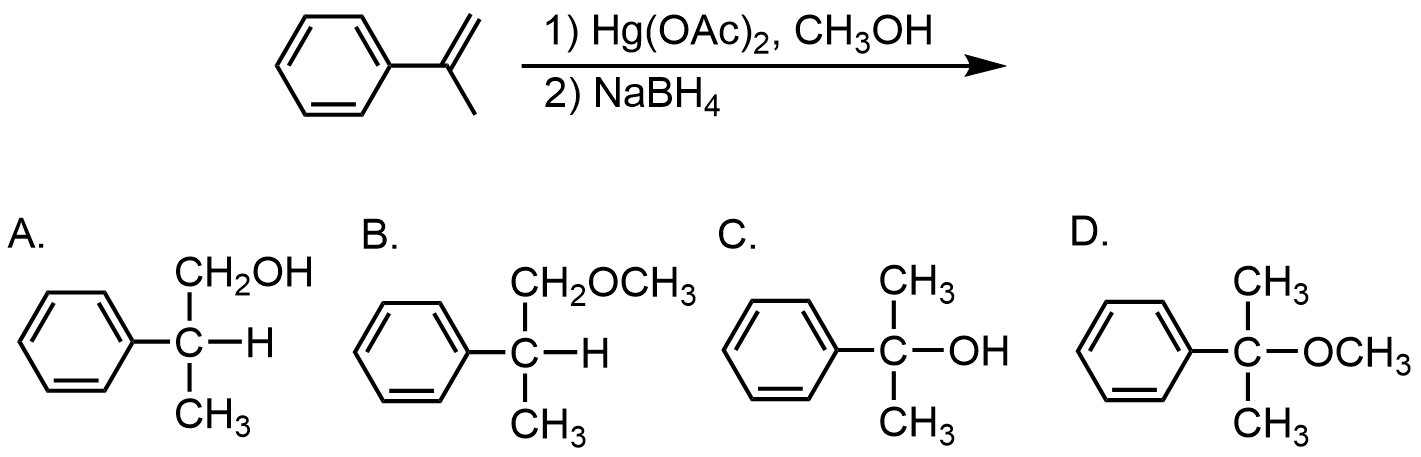
\includegraphics[scale=0.38, valign=c]{./Figure/2018/2018_4_1.png}
    \item 下列化合物不具有手性的是
    
    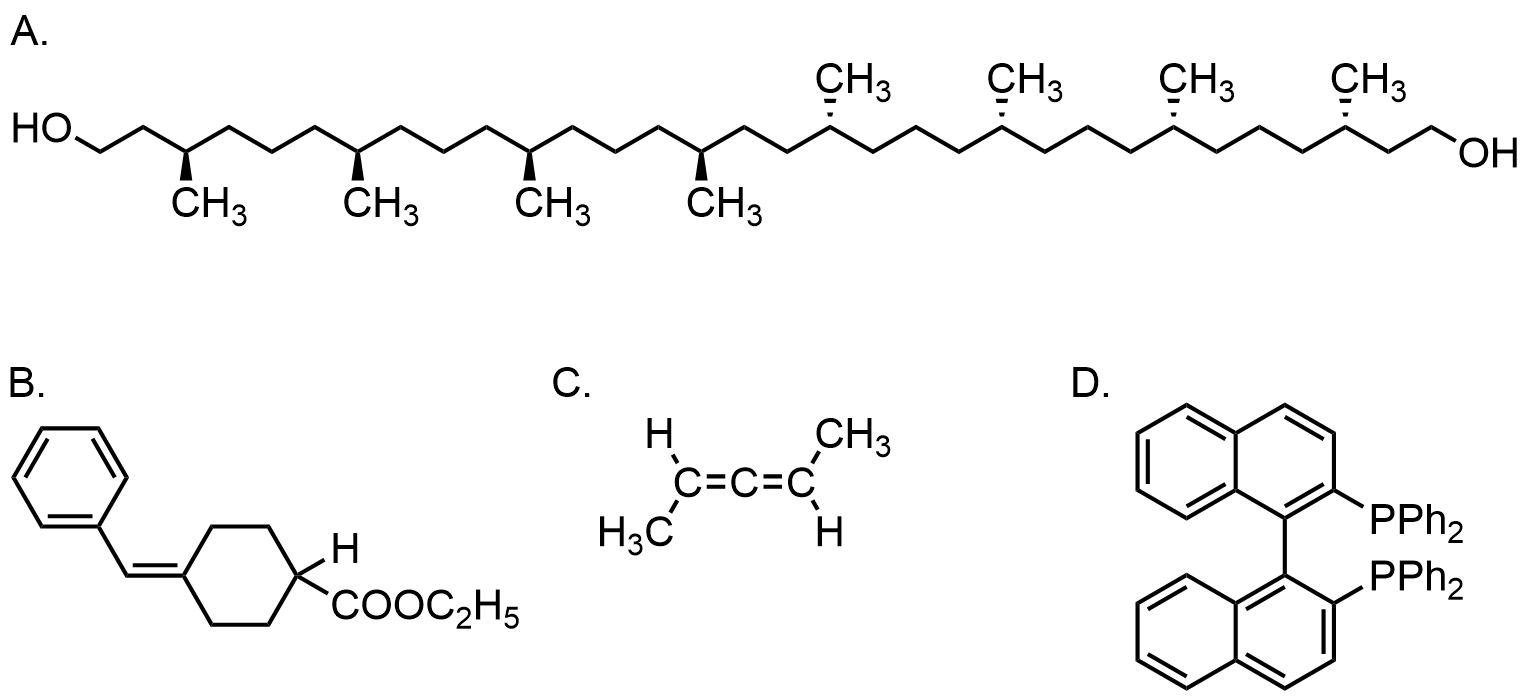
\includegraphics[scale=0.38, valign=c]{./Figure/2018/2018_4_2.png}
    \item 下列羰基化合物与\ce{CH3MgI}反应时，慢反应一步活化能最低的是
    
    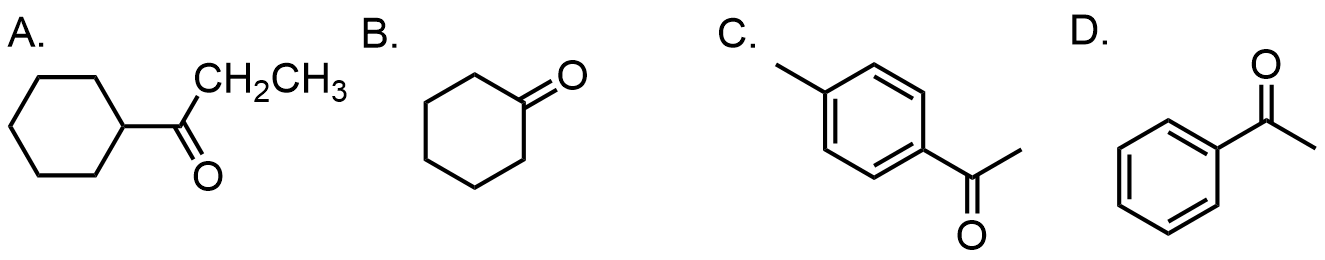
\includegraphics[scale=0.38, valign=c]{./Figure/2018/2018_4_3.png}
    \item 下列共振式对杂化体的贡献最大的是
    
    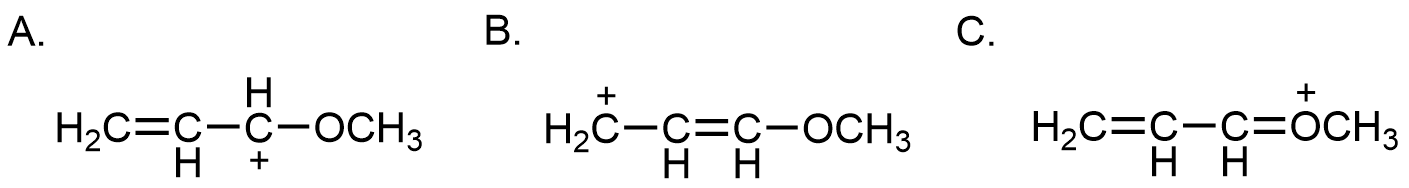
\includegraphics[scale=0.38, valign=c]{./Figure/2018/2018_4_4.png} 
    \item 下列化合物发生$S_{N}1$反应时速度最快的是
    
    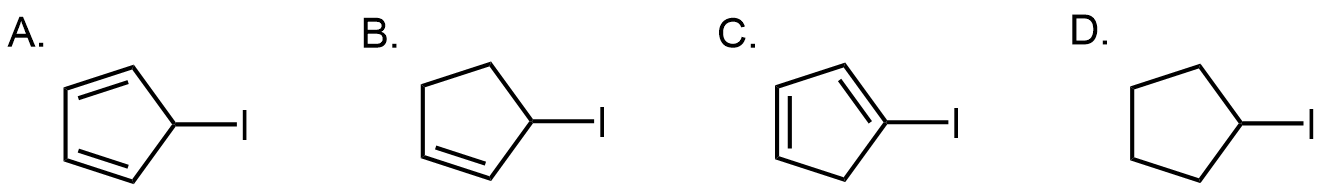
\includegraphics[scale=0.38, valign=c]{./Figure/2018/2018_4_5.png} 
    \item 下列化合物不具有芳香性的是
    
    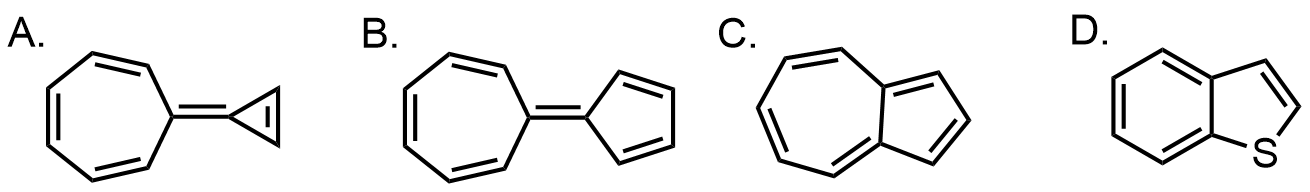
\includegraphics[scale=0.38, valign=c]{./Figure/2018/2018_4_6.png}
    \item 下列化合物碱性最强的是
    
    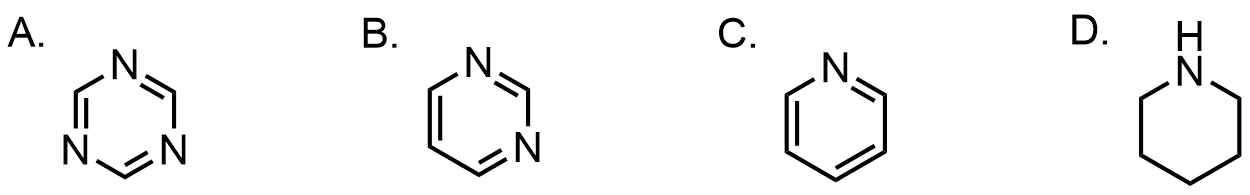
\includegraphics[scale=0.38, valign=c]{./Figure/2018/2018_4_7.png}
    \item 下列化合物亲核性最强的是
    \begin{tasks}(2)
        \task \ce{CH3CH2CH2COO-}
        \task \ce{CH3CH2CH2CH2S-}
        \task \ce{CH3CH2CH2CH2O-}
        \task \ce{CH3CH2CH2CH2SH}
    \end{tasks}
    \item 给出如下反应的主产物
    
    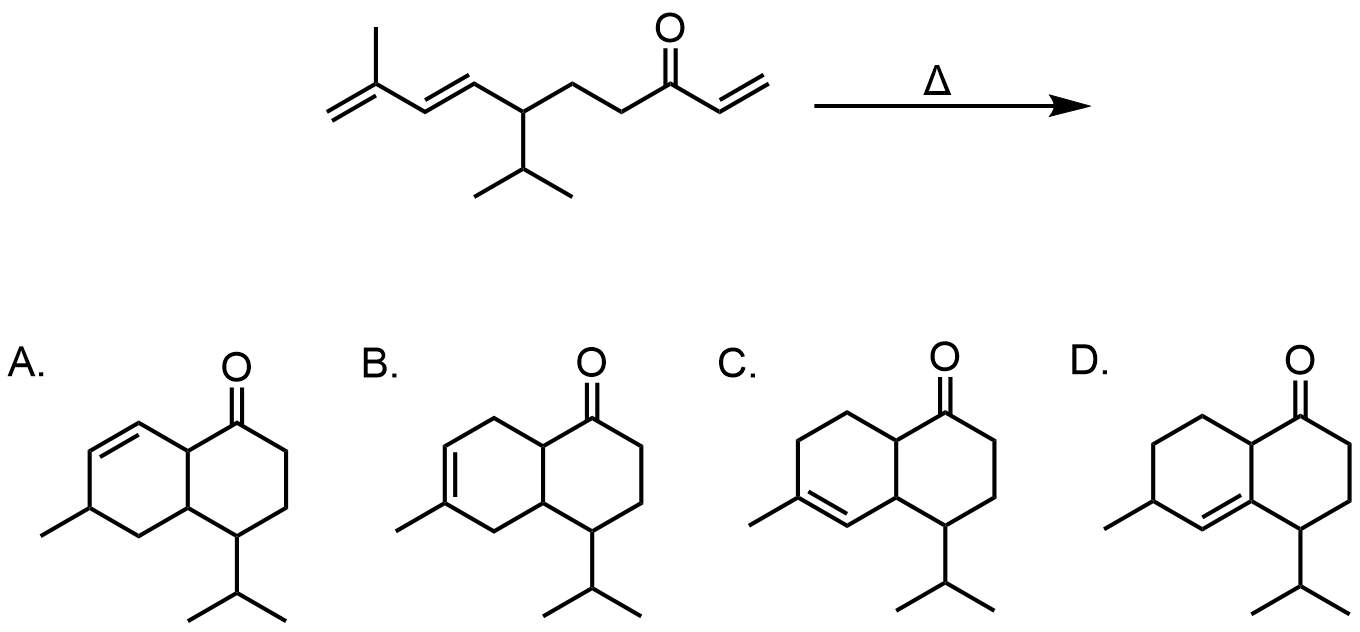
\includegraphics[scale=0.38, valign=c]{./Figure/2018/2018_4_9.png}
    \item 不能在氨基钠/液氨中生成苯胺衍生物的是
    
    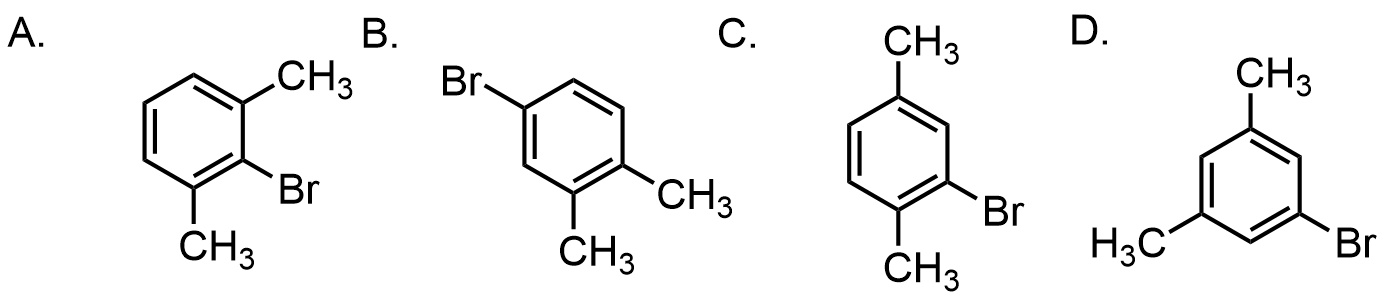
\includegraphics[scale=0.38, valign=c]{./Figure/2018/2018_4_10.png}
    \item 下列化合物中酸性最强的是

    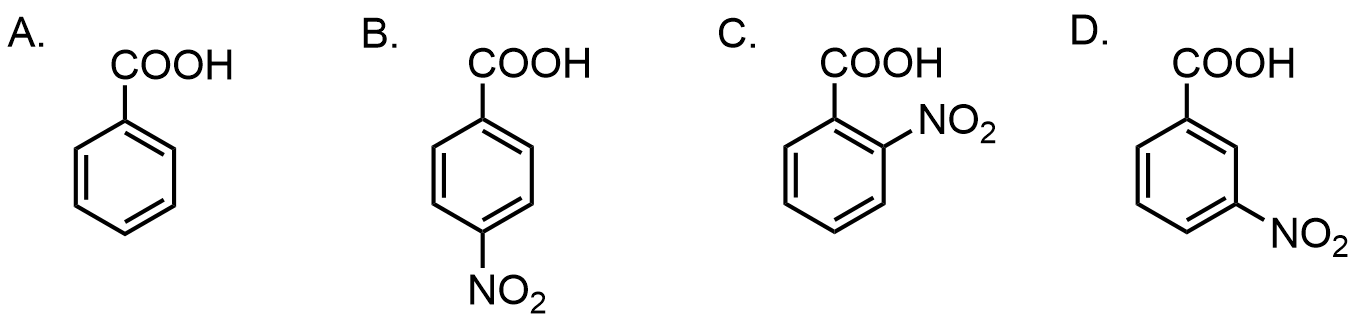
\includegraphics[scale=0.38, valign=c]{./Figure/2018/2018_4_11.png}
    \item 不能与饱和\ce{NaHSO3}反应的是
    \begin{tasks}(4)
        \task 苯甲醛
        \task 环己酮
        \task $\beta$-甲基环己酮
        \task D-(+)-果糖
    \end{tasks}
    \item 下列溶剂中属于质子溶剂的是
    \begin{tasks}(4)
        \task THF
        \task t-BuOH
        \task DMSO
        \task 吡啶
    \end{tasks}
    \item 下列化合物烯醇式含量最高的是
    \begin{tasks}(2)
        \task \ce{CH3COCH2COCF3}
        \task \ce{CH3COCH2COCCl3}
        \task \ce{CH3COCH2COCH3}
        \task \ce{CH3COCH2COOC2H5}
    \end{tasks}
    \item 不能用无水氯化钙干燥的有机物是
    \begin{tasks}(4)
        \task 1-溴丁烷
        \task 2-甲基-2-丁醇
        \task 二丁醚
        \task 硝基苯
    \end{tasks}
\end{enumerate}

\vspace{0.5cm}
\noindent\textbf{二、完成反应(50 pts.)}

\begin{enumerate}[label=\arabic*., itemsep=3ex]
    \item 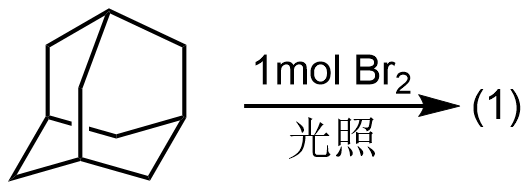
\includegraphics[scale=0.3, valign=c]{./Figure/2018/2018_1_1.png} 
    \item 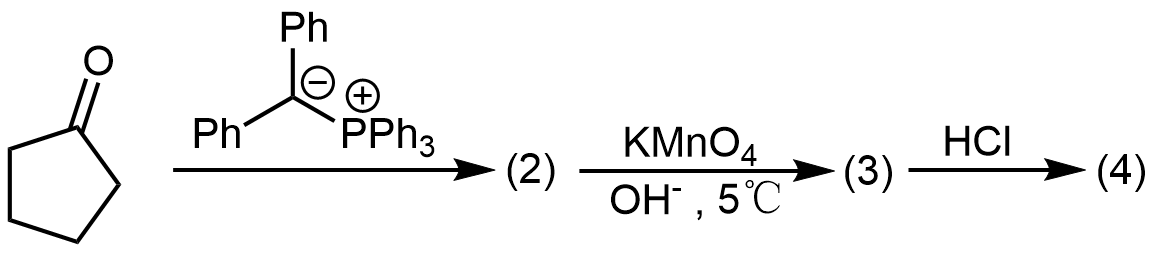
\includegraphics[scale=0.3, valign=c]{./Figure/2018/2018_1_2.png}
    \item 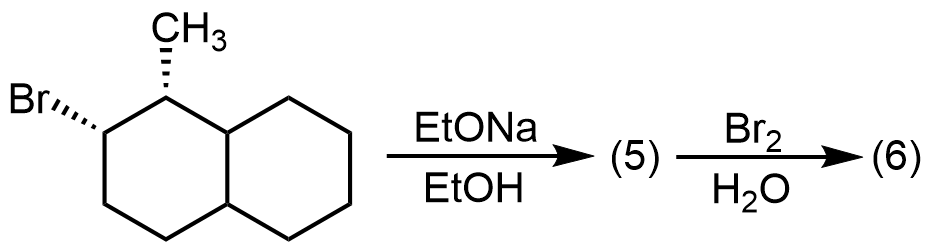
\includegraphics[scale=0.3, valign=c]{./Figure/2018/2018_1_3.png}
    \item 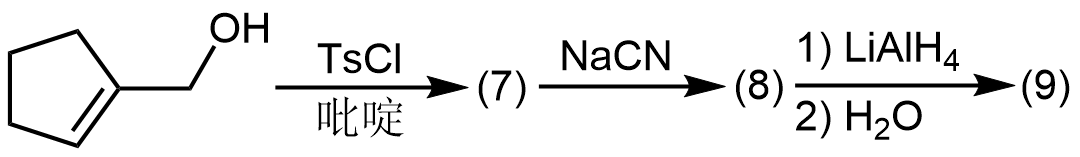
\includegraphics[scale=0.3, valign=c]{./Figure/2018/2018_1_4.png}
    \item 请画出如下化合物的优势构象
    
    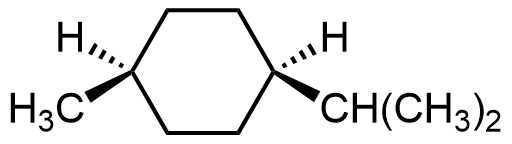
\includegraphics[scale=0.3, valign=c]{./Figure/2018/2018_1_5.png}
    \item 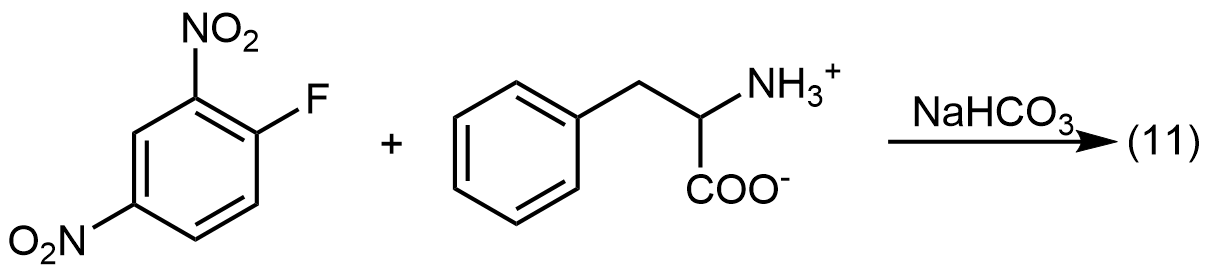
\includegraphics[scale=0.3, valign=c]{./Figure/2018/2018_1_6.png}
    \item 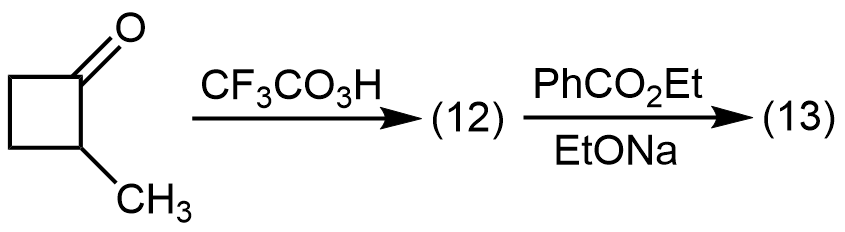
\includegraphics[scale=0.3, valign=c]{./Figure/2018/2018_1_7.png}
    \item 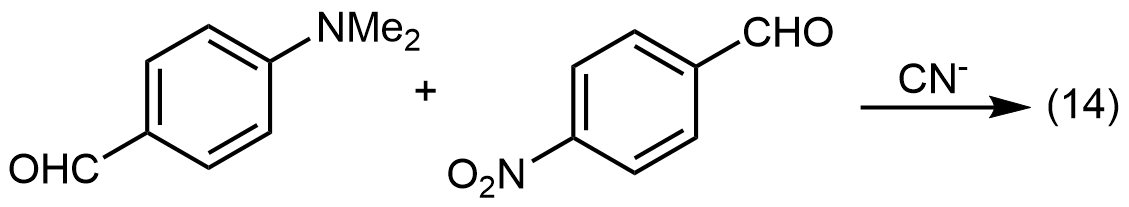
\includegraphics[scale=0.3, valign=c]{./Figure/2018/2018_1_8.png}
    \item 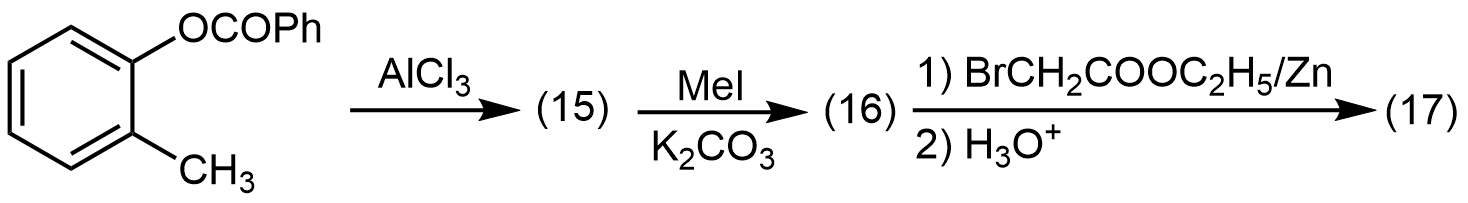
\includegraphics[scale=0.3, valign=c]{./Figure/2018/2018_1_9.png}
    \item 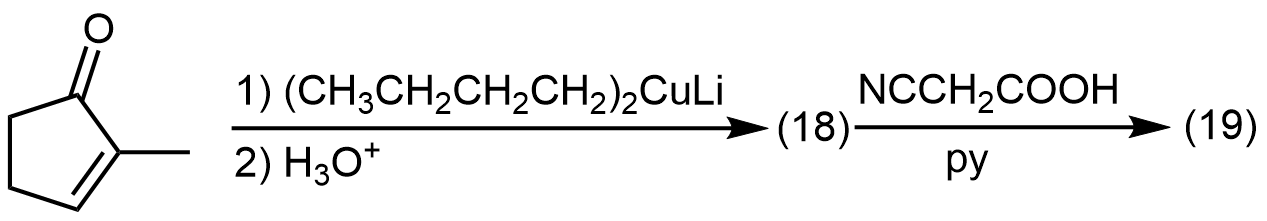
\includegraphics[scale=0.3, valign=c]{./Figure/2018/2018_1_10.png}
    \item 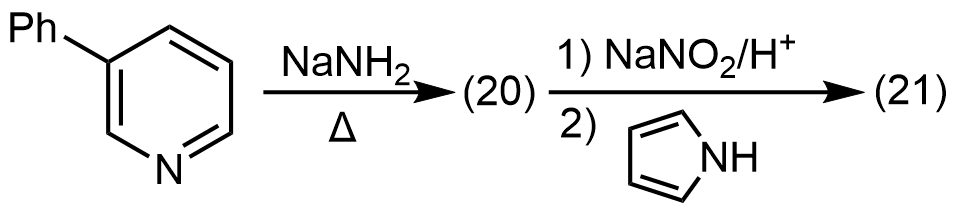
\includegraphics[scale=0.3, valign=c]{./Figure/2018/2018_1_11.png}
    \item 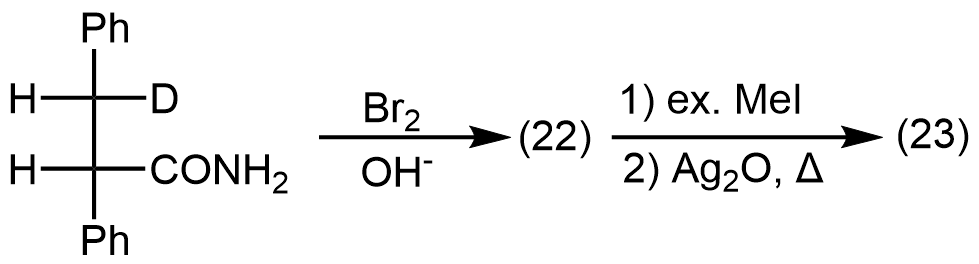
\includegraphics[scale=0.3, valign=c]{./Figure/2018/2018_1_12.png}
    \item 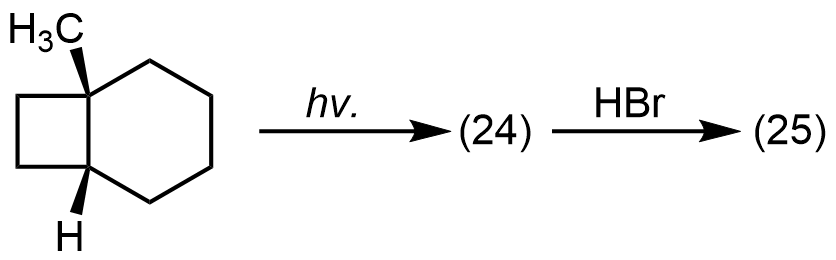
\includegraphics[scale=0.3, valign=c]{./Figure/2018/2018_1_13.png}


\end{enumerate}

\vspace{0.5cm}
\noindent\textbf{三、机理题(28 pts.)}

\begin{enumerate}[label=\arabic*., start=1, itemsep=1.5ex]
    \item 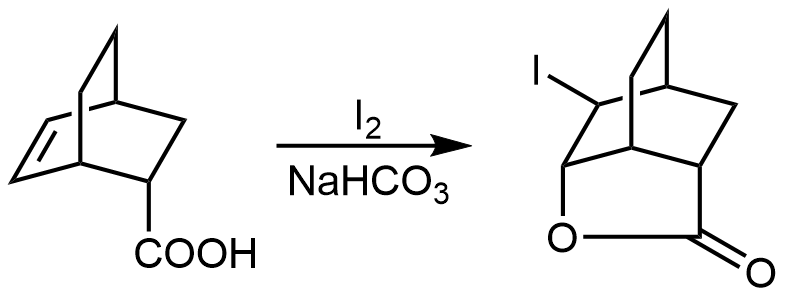
\includegraphics[scale=0.3, valign=c]{./Figure/2018/2018_2_1.png}
    \item 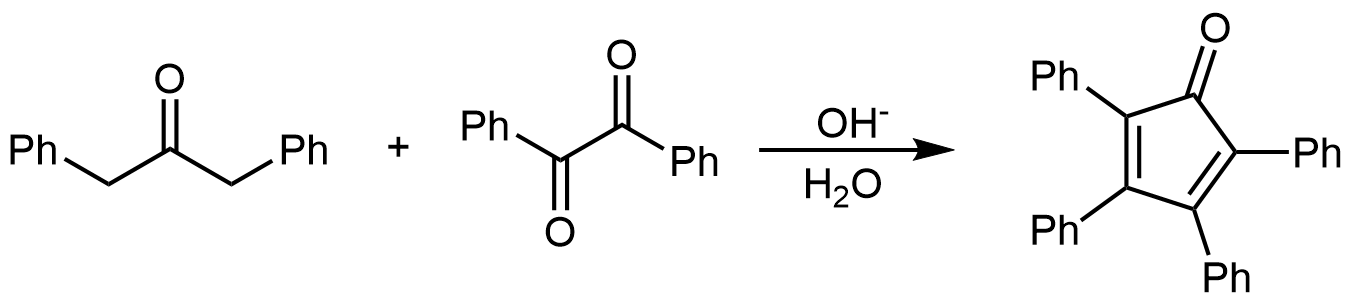
\includegraphics[scale=0.3, valign=c]{./Figure/2018/2018_2_2.png}
    \item 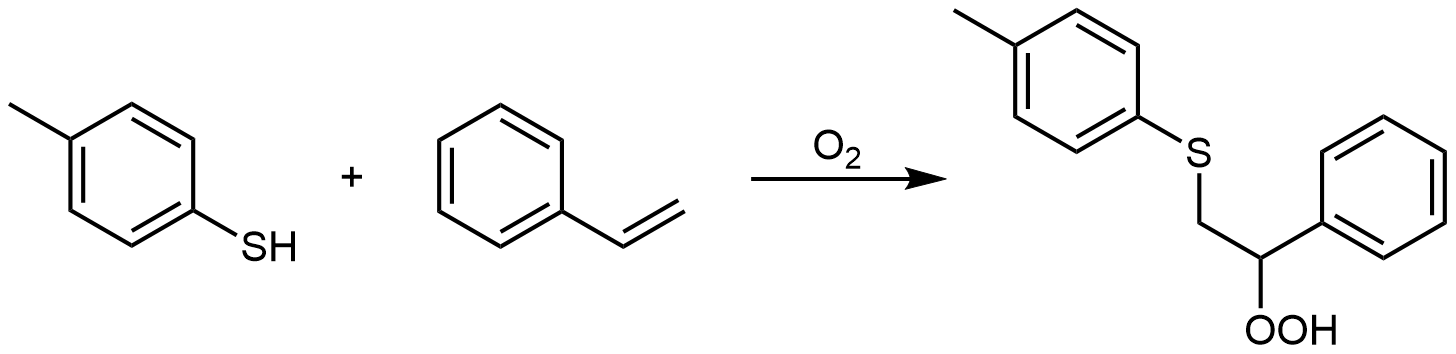
\includegraphics[scale=0.3, valign=c]{./Figure/2018/2018_2_3.png}
    \item 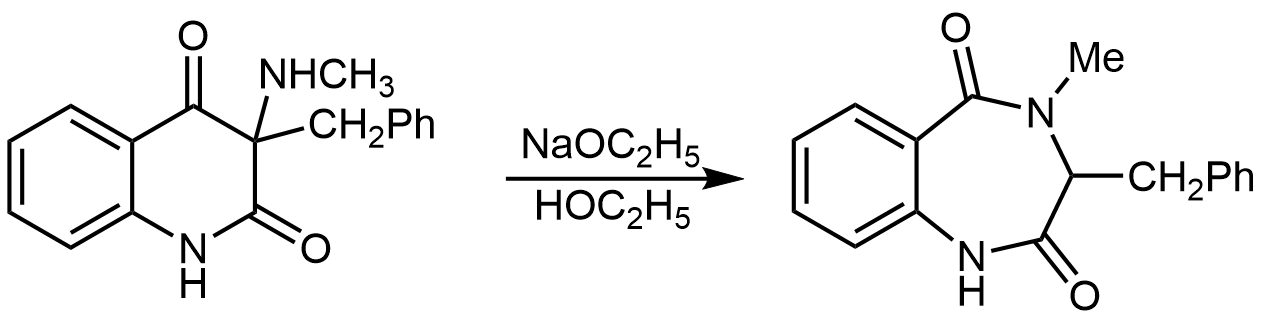
\includegraphics[scale=0.3, valign=c]{./Figure/2018/2018_2_4.png}
\end{enumerate}

\vspace{0.5cm}
\noindent\textbf{四、合成题(42 pts.)}

\begin{enumerate}[label=\arabic*., start=1, itemsep=1.5ex]

    \begin{figure}[htbp]
        \centering
        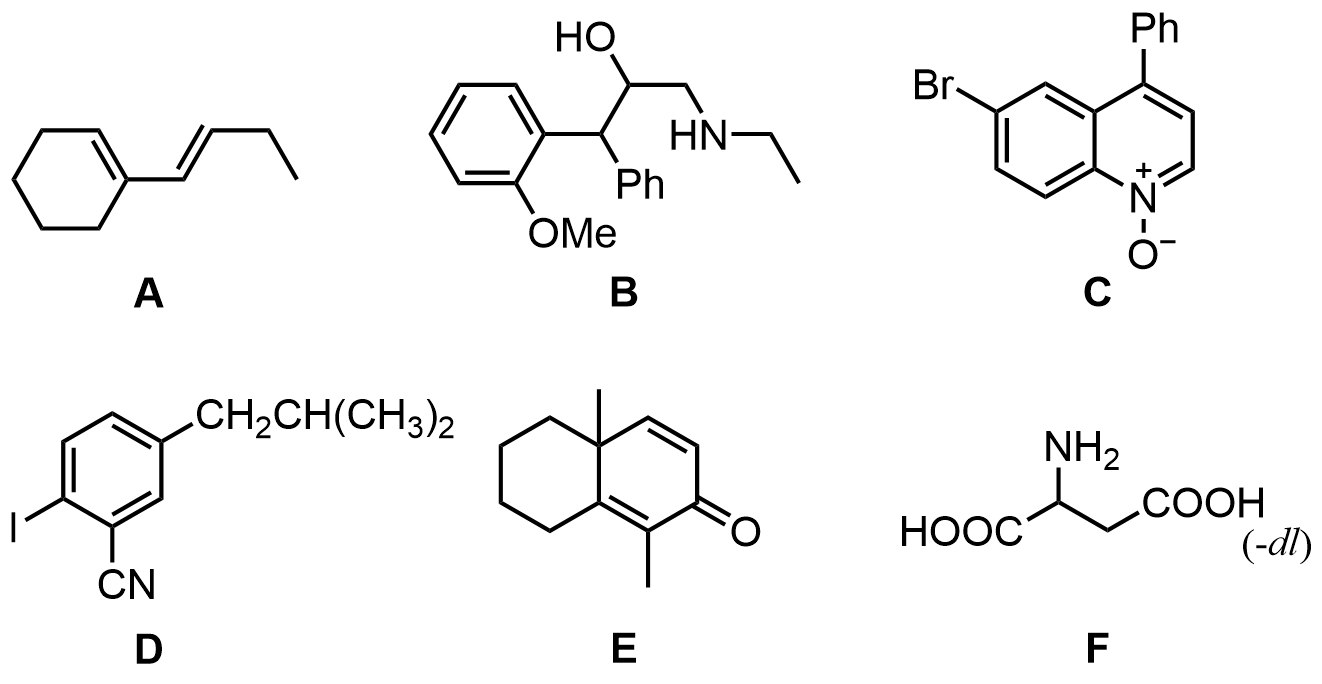
\includegraphics[scale=0.38]{./Figure/2018/2018_3.png}
    \end{figure}
    \item 以乙炔为唯一有机原料合成\textbf{A}
    \item 以苯、小于等于3个碳的有机物合成\textbf{B}
    \item 以苯、小于等于3个碳的有机物合成\textbf{C}
    \item 以苯、小于等于4个碳的有机物合成\textbf{D}
    \item 以环己酮、小于等于3个碳的有机物合成\textbf{E}
    \item 以邻苯二甲酰亚胺、丙二酸二乙酯、小于等于4个碳的有机物合成\textbf{F}
\end{enumerate}

\vspace{0.5cm}
\noindent\textbf{五、实验题 略}